% Name: Dragon curve
% Description: The Heighway dragon after twelve folds: a single path of right-angle turns that never crosses itself.
% Tags: dragon curve, Heighway dragon, fractal, L-system

\usetikzlibrary{lindenmayersystems}

\pgfdeclarelindenmayersystem{Dragon curve}{
  \rule{X -> X+YF+}
  \rule{Y -> -FX-Y}}

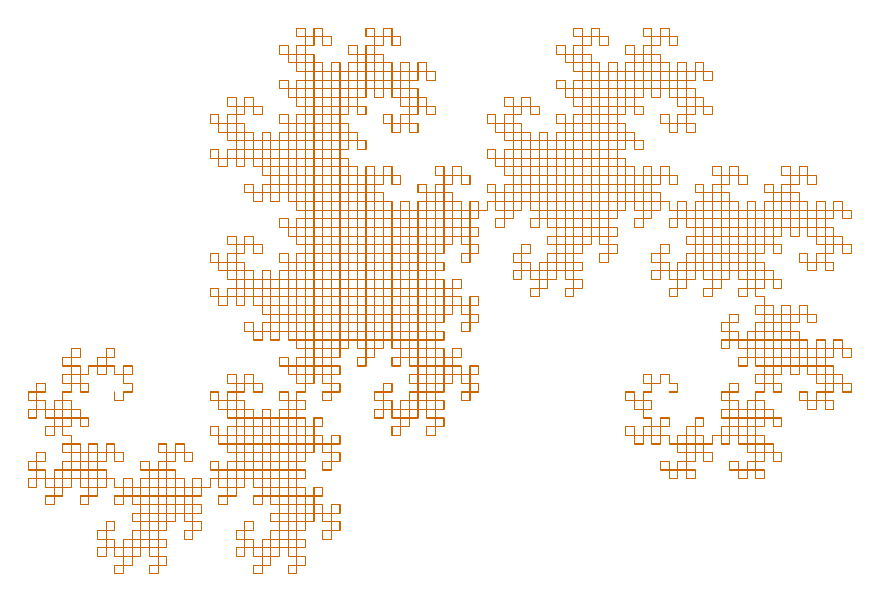
\begin{tikzpicture}
  \draw[orange!80!black, line join=round, line cap=round, lindenmayer system={Dragon curve, axiom=FX, order=12, angle=90, step=1.1mm}] lindenmayer system;
\end{tikzpicture}
